\section{One periodic word synchronizes a finite interval}
\label{sec:synchronization}

Fix a finite set of seeds. We seek a periodic word that applies the same
letter to every seed at each step. The positive-coordinate maps from
\eqref{eq:positive-switch} satisfy
\[
 \{T(z),U(z)\}
 =\left\{\left\lceil\frac z2\right\rceil,
          \left\lceil\frac{3z}2\right\rceil\right\}.
\]
Write $D(z)$ and $A(z)$ for the two values in the displayed order.
The letter that gives $D(z)$ depends on the parity of $z$.

For a single trajectory, Vasilyev's Theorem~4.1(a) gives steering by
upward and downward edges, and Proposition~4.3 allows a policy depending
on the current integer \cite{vasilyev-2026}. For an ensemble, one letter
must serve all current parities. We also require a bounded reference
trajectory and synchronization from every launch phase.

\subsection{A bounded reference and a common reset word}

Keep a distinguished reference $r$ in $\{1,2,3\}$ using only the
following allowed transitions:
\begin{equation}\label{eq:reference-controller}
 1\xrightarrow{T}2,\quad 1\xrightarrow{U}1,\quad
 2\xrightarrow{T}1,\quad 2\xrightarrow{U}3,\quad
 3\xrightarrow{U}2.
\end{equation}
In particular, $T$ is forbidden at reference value $3$.

Pairwise merger implies a finite-set reset in a deterministic automaton
\cite[Theorem~2]{cerny-1964}. Here a comparison value can leave the
initial interval. We prove a merger for every such value while the
reference stays in $\{1,2,3\}$.

\begin{lemma}[Protected merger]\label{lem:protected-merger}
For every finite set $S$ of positive integers containing a reference
$r\in\{1,2,3\}$, an allowed finite word sends all members of $S$
to the reference. The word may be chosen to finish with reference
value $1$.
\end{lemma}
\begin{proof}
First merge the reference with one comparison state $M$.
If $M\ge6$, choose the letter that applies $D$ to $M$. This letter
is allowed unless $r=3$ and $M$ is even. In the exceptional case,
apply $U$, obtaining reference $2$ and comparison value $3M/2$,
and then apply whichever letter decreases that comparison value.
Both letters are allowed at reference $2$. After these two steps
the comparison value is at most $3M/4+1/2<M$.
Otherwise one step gives $D(M)<M$. Consequently repeated blocks of
one or two allowed letters either produce a merger or bring $M$
below $6$.

For the remaining distinct ordered pairs the following words give
mergers. Letters are read from left to right.
\begin{center}
\begin{tabular}{ccl}
\hline
Reference & Comparison values & Word\\
\hline
$1$ & $2,5$ & $UTU$\\
$1$ & $3$ & $TU$\\
$1$ & $4$ & $T$\\
$2$ & $1,3,4$ & $TUTU$\\
$2$ & $5$ & $U$\\
$3$ & $1,2,5$ & $UTUTU$\\
$3$ & $4$ & $UTTU$\\
\hline
\end{tabular}
\end{center}
These entries are verified by substituting the two parity formulas
for $T$ and $U$; no entry applies $T$ at reference $3$.
Apply a merger word to the entire current set. The reference remains
in the set, previously merged states remain merged, and its
cardinality drops whenever it is not a singleton. Finitely many
such operations synchronize $S$. A final $T$ from reference $2$,
or $UT$ from reference $3$, brings the common value to $1$.
\end{proof}

\subsection{A ten-step reset worked in full}

Start with reference $r_0=1$ and the positive-coordinate ensemble
$S_0=\{1,2,3,4,5,6\}$. Apply the same chronological word
\begin{equation}\label{eq:small-reset-word}
 w=U\,T\,T\,U\,T\,U\,U\,U\,U\,T
\end{equation}
to every member. The complete image sets are
\begin{center}\small
\begin{tabular}{rcrl}\toprule
Time $k$ & Next letter & Reference $r_k$ & Distinct image set $S_k$\\\midrule
0&$U$&1&$\{1,2,3,4,5,6\}$\\
1&$T$&1&$\{1,2,3,6,9\}$\\
2&$T$&2&$\{1,2,3,5,14\}$\\
3&$U$&1&$\{1,2,5,7,8\}$\\
4&$T$&1&$\{1,3,4,12\}$\\
5&$U$&2&$\{2,5,6\}$\\
6&$U$&3&$\{3,9\}$\\
7&$U$&2&$\{2,5\}$\\
8&$U$&3&$\{3\}$\\
9&$T$&2&$\{2\}$\\
10&--&1&$\{1\}$\\\bottomrule
\end{tabular}
\end{center}
The first $U$ merges $2$ and $5$ at $3$ while sending $6$ to $9$.
At time eight the same collision leaves a singleton. The last two
letters return its value to $1$. Every transition respects the reference
rule.

\begin{figure}[t]
\centering
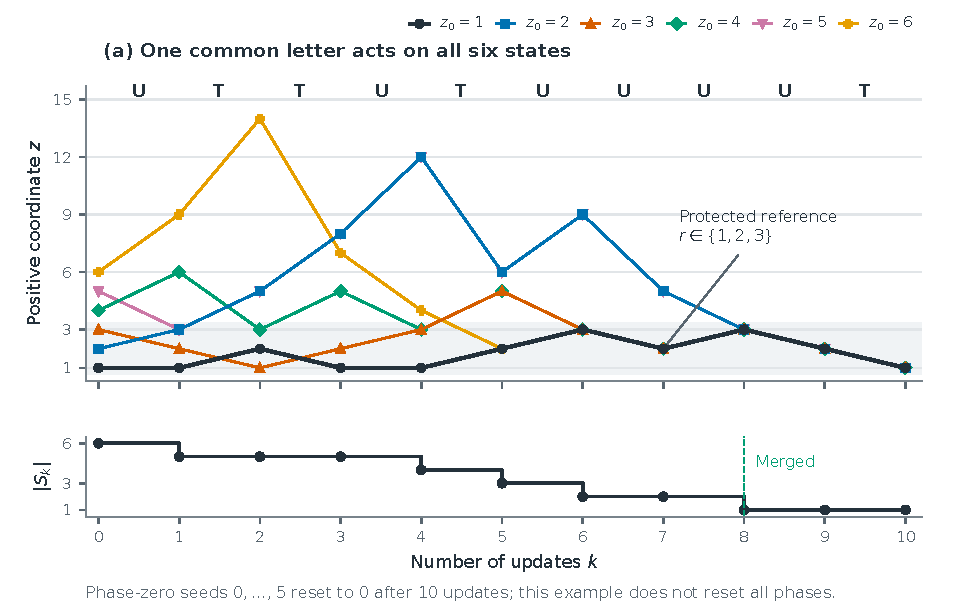
\includegraphics[width=\linewidth]{figures/synchronization.pdf}
\caption{Exact common control for \eqref{eq:small-reset-word}.
The six initial positive-coordinate values receive the same letter
at every time. Their tracks merge into the protected reference;
the distinct image count falls from six to one. The first merger
of the entire ensemble occurs at time eight, and the reference
returns to one at time ten.}
\label{fig:common-reset}
\end{figure}

Set $h_i=0$ for a $U$ letter and $h_i=1$ for a $T$ letter, with
the height read cyclically. For this example,
\begin{align}
 h&=(0,1,1,0,1,0,0,0,0,1),\nonumber\\
 d&=(1,0,-1,1,-1,0,0,0,1,-1),\label{eq:small-reset-forcing}\\
 b&=(0,1,2,0,1,1,2,1,2,2).\nonumber
\end{align}
Here $d_i=h_{i+1}-h_i$ and $b_i=r_i-1+h_i$.
Direct substitution gives $T(b_i)+d_i=b_{i+1}$, including the
last-to-first update. The three positive and three negative impulses
alternate, so the forcing is conservative and admissible. Its
primitive period is ten: a shorter period dividing ten would repeat
a shorter block either twice or five times, inconsistent with its
three positive impulses.

At phase zero the coordinate change is $z=n+1$. Thus the six
physical seeds $0,1,2,3,4,5$ correspond exactly to $S_0$ and all
satisfy
\begin{equation}\label{eq:small-physical-reset}
 F_{d,0}^{(10)}(n)=0\qquad(0\le n\le5).
\end{equation}
Repeating the word then follows the displayed response $b$.
The chosen launch phase is essential to this particular reset:
seed $5$ launched at phase one has value $3$ after ten updates,
whereas $b_1=1$. Thus \eqref{eq:small-physical-reset} does not
already give the one-period all-phase conclusion. The rotation
argument below supplies the additional condition needed to obtain
that stronger property for a suitable longer word.

The same construction gives periodic capture of any prescribed finite
set at one chosen phase. Start with
reference $1$, height zero, and the transformed values $n+1$ of the
specified nonnegative physical seeds. Apply an initial $U$, use
Lemma~\ref{lem:protected-merger}, and close the binary height word
back at zero. The period map sends every specified seed to zero.
During the reference response, the physical value is
$b=r-1+h\in B=\{0,1,2\}$: the only combination that would give
$b=3$ is $r=3,h=1$, which is forbidden by
\eqref{eq:reference-controller}. The next argument controls all
rotations and gives a logarithmic period bound.

\subsection{An explicit contraction estimate}

Sequential protected mergers prove existence, but during one merger
the other comparison values may grow. A period bound needs a quantity
that controls the entire current ensemble at once. A fractional power
is useful because it discounts the cost of an occasional growing step.
For example, strict concavity gives
\[
 \frac12\left[\left(\frac z2\right)^{1/4}
              +\left(\frac{3z}{2}\right)^{1/4}\right]
 <z^{1/4},
\]
whereas the corresponding average of the two values themselves is
exactly $z$. The reference constraint prevents us from choosing the
two letters with equal probability at every reference state. The
weights below compensate for that constraint.

For a finite set $S$ of \emph{distinct} positive integers containing
$r$, put
\begin{equation}\label{eq:sync-potential}
 P(r,S)=g_r\sum_{z\in S}z^{1/4},\qquad
 (g_1,g_2,g_3)=\left(\frac{19}{20},1,\frac{111}{100}\right).
\end{equation}
Choose the next letter with probabilities
\begin{equation}\label{eq:reference-probabilities}
 \mathbb P(T\mid r=1)=\frac{19}{39},\quad
 \mathbb P(T\mid r=2)=\frac{111}{206},\quad
 \mathbb P(T\mid r=3)=0.
\end{equation}
The same chosen letter acts on every member of $S$, and duplicate
images are discarded. Randomness is used only for an existence
argument about finite words.

There is a related random-map synchronization theorem of Yano and
Yasutomi: a finite irreducible aperiodic Markov chain admits a choice
of mapping law with synchronizing support
\cite{yano-yasutomi-2011}. In the present process, the maps
and their simultaneous action on the integer ensemble are prescribed.
Consequently, mixing of the finite reference chain alone does not
establish synchronization of the ensemble; its merger and drift
estimates must be proved for this common action.

The probabilities can be read directly from the reference weights.
At reference one, a $T$ step moves to reference two and a $U$ step
stays at one. Choosing $p_1=\mathbb P(T\mid r=1)$ to satisfy
\[
 p_1g_2=(1-p_1)g_1
\]
gives $p_1=g_1/(g_1+g_2)=19/39$. At reference two, the two
destinations are one and three. Balancing their contributions gives
\[
 p_2g_1=(1-p_2)g_3,
 \qquad p_2=\frac{g_3}{g_1+g_3}=\frac{111}{206}.
\]
Thus the coefficient of a shrinking branch equals the coefficient
of a growing branch, whichever letter provides it for a particular
input parity. At reference three the only letter is $U$, but its
destination has the smaller weight $g_2$. The chosen ratio
$g_3/g_2=111/100$ exceeds the fourth-root growth factor
$(3/2)^{1/4}$, allowing contraction even in that worst parity case.

Removing duplicate images is also part of the estimate. Once two
initial seeds share a current value, every remaining common letter
acts identically on them. They impose one remaining synchronization
condition, so the potential counts their common value once. In the
worked example, the six tracked labels eventually contribute just
one term to the potential, while the reference continues around its
small allowed state space.

\begin{lemma}[Fractional-power drift]\label{lem:protected-drift}
For this process,
\begin{equation}\label{eq:sync-drift}
 \mathbb E[P(r',S')\mid r,S]
 \le\frac{999}{1000}P(r,S)
    +\left(\frac{25P(r,S)}{19}\right)^{1/5}.
\end{equation}
In particular, with $K_0=16000$ and $\rho=1999/2000$,
\begin{equation}\label{eq:sync-geometric-drift}
 P(r,S)\ge K_0\quad\Longrightarrow\quad
 \mathbb E[P(r',S')\mid r,S]\le\rho P(r,S).
\end{equation}
\end{lemma}
\begin{proof}
Write $a=2^{-1/4}$ and $b=(3/2)^{1/4}$. For an even input the
two branch values are exactly $z/2$ and $3z/2$. For an odd input
they have an additional $1/2$. Ignoring this additive correction
temporarily, the expected gain of $g_{r'}z'^{1/4}$ relative to
$g_rz^{1/4}$ is bounded, for $r=1,2,3$, respectively by
\[
 \frac{20(a+b)}{39},\qquad
 \frac{10545(a+b)}{20600},\qquad
 \frac{100b}{111}.
\]
In the first two expressions the weighted probabilities of the two
letters are equal, so the bound is independent of the input parity.
The third is the larger of the two possible parity gains.
The rational inequalities $a<841/1000$ and $b<1107/1000$ follow
by taking fourth powers. They give the respective upper bounds
\[
 \frac{974}{975},\qquad
 \frac{1027083}{1030000},\qquad
 \frac{369}{370},
\]
each strictly below $999/1000$.

For $c\in\{1/2,3/2\}$, concavity gives
\[
 (cz+1/2)^{1/4}-(cz)^{1/4}
 \le\frac18(cz)^{-3/4}.
\]
Multiplication by $g_{r'}\le111/100$ bounds the correction by
$(111/800)2^{3/4}z^{-3/4}<z^{-3/4}/4$.
The last inequality follows from $8\cdot111^4<200^4$.
Discarding duplicate images can only reduce the potential.

If $m=|S|$ and its members are listed increasingly, the $j$th is
at least $j$. Comparison with integrals yields
\[
 \sum_{z\in S}z^{-3/4}
 \le\sum_{j=1}^{m}j^{-3/4}\le4m^{1/4},\qquad
 \sum_{z\in S}z^{1/4}\ge\sum_{j=1}^{m}j^{1/4}
 \ge\frac45m^{5/4}.
\]
Thus $P\ge(19/25)m^{5/4}$, and the total additive error is at
most $m^{1/4}\le(25P/19)^{1/5}$. This proves
\eqref{eq:sync-drift}. For $P\ge16000$,
$(25P/19)^{1/5}\le P/2000$: after taking fifth powers it is
enough that $19P^4\ge25\cdot2000^5$, which already holds at
$P=16000$ and is preserved as $P$ increases.
\end{proof}

\subsection{A uniform tail for synchronization}

The drift bounds the waiting time until the ensemble has small potential.
There Lemma~\ref{lem:protected-merger} gives a positive probability of
a reset in bounded time. After a failed trial the same drift bounds the
time to the next trial. This applies the drift and minorization method
\cite[Theorem~12]{rosenthal-1995} to the whole ensemble under a common
sequence of letters.

\begin{lemma}[Exponential synchronization tail]\label{lem:sync-tail}
Let $\tau$ be the first time the ensemble is the singleton containing
the reference. There are absolute constants $c,C_1>0$ such that
\begin{equation}\label{eq:sync-tail}
 \mathbb P_{r,S}(\tau>t)
 \le C_1\bigl(1+P(r,S)\bigr)e^{-ct}
 \qquad(t\in\N).
\end{equation}
\end{lemma}
\begin{proof}
Let $\mathcal C=\{(r,S):P(r,S)<K_0\}$. It is a finite set of
ensemble states: every member of such an $S$ is at most
$K=\lceil(320000/19)^4\rceil$. If $\sigma$ is the first entrance
time into $\mathcal C$, the killed version of
\eqref{eq:sync-geometric-drift} gives
\[
 \mathbb E[P(r_t,S_t)\mathbf1_{\{\sigma>t\}}]
 \le\rho^t P(r,S),\qquad
 \mathbb P(\sigma>t)\le\frac{P(r,S)}{K_0}\rho^t.
\]
For $0<\beta_0<-\log\rho$, the tail-sum identity for a
nonnegative integer-valued stopping time therefore gives
\begin{equation}\label{eq:entrance-moment}
 \mathbb E e^{\beta_0\sigma}
 \le1+a_0P(r,S),\qquad
 a_0=\frac{e^{\beta_0}-1}{K_0(1-\rho e^{\beta_0})}.
\end{equation}
In particular the entrance time is finite almost surely.

For each possible reference value, apply
Lemma~\ref{lem:protected-merger} to the entire finite interval
$\{1,\ldots,K\}$. Pad the resulting words by $U$ at reference
$1$ so that they have one common length $m_0$. Every positive
allowed letter probability in \eqref{eq:reference-probabilities}
is at least $95/206$. A trial of $m_0$ steps begun in
$\mathcal C$ therefore succeeds in synchronizing with conditional
probability at least
$\varepsilon=(95/206)^{m_0}>0$.

After any trial, define $D$ to be its length $m_0$ plus the
subsequent time needed to return to $\mathcal C$. This can be
defined whether or not the trial succeeds. The potential at the
end of a trial is uniformly bounded over initial states in
$\mathcal C$: each individual output is at most twice its input
at each step, the number of image points cannot increase, and the
three reference weights are bounded away from zero. Equation
\eqref{eq:entrance-moment} consequently implies
\[
 M_0:=\sup_{x\in\mathcal C}\mathbb E_x e^{\beta_0D}<\infty.
\]
Let $H$ be the event that synchronization has not occurred by the
end of the trial. Then $\mathbb P_x(H)\le1-\varepsilon$.
For $0<\theta<1$, H\"older's inequality gives
\[
 \mathbb E_x[e^{\theta\beta_0D}\mathbf1_H]
 \le M_0^\theta(1-\varepsilon)^{1-\theta}.
\]
Choose $\theta>0$ small enough that the right side is some
$\kappa<1$, and put $\beta=\theta\beta_0$.

Repeat the trial after each failed trial and return to
$\mathcal C$. The conditional failure bound ensures eventual
success almost surely. The strong Markov property and the preceding
weighted failure estimate bound the contribution of success on
trial $j$ to the exponential moment by
$e^{\beta m_0}\kappa^{j-1}$. Summing over $j\ge1$ and accounting
for the initial entrance time with
\eqref{eq:entrance-moment} gives
$\mathbb E e^{\beta\tau}\le C(1+P(r,S))$ for an absolute
$C$. Markov's inequality proves \eqref{eq:sync-tail}.
The argument uses conditional bounds and the strong Markov property;
it makes no independence assumption between different trials.
\end{proof}

For an interval ensemble $\{1,\ldots,N+2\}$, the initial potential
is at most $(111/100)(N+2)^{5/4}$. Consequently, for
$0<\varepsilon<1$, the probability of failure at a single chosen
phase is at most $\varepsilon$ whenever
\[
 t\ge\left\lceil\frac1c\left(\frac54\log(N+2)
                    +\log\frac1\varepsilon+C_4\right)\right\rceil
\]
for an absolute constant $C_4$.

\subsection{Closing the clock and treating every launch phase}

A closed reference path gives a periodic response. To reset the seeds
from every phase, each rotation of its label word must synchronize the
transformed seeds at that phase.

\begin{theorem}[Logarithmic all-phase synchronization]
\label{thm:all-phase-synchronization}
There exist absolute finite constants $C,C_0$ with the following
property. For every integer $N\ge1$ there is a nonzero conservative
admissible forcing word of odd prime primitive period $p$, with
\begin{equation}\label{eq:sync-period-order}
 \left\lceil\log_2(N+1)\right\rceil
 \le p\le C\log(N+2)+C_0,
\end{equation}
and a phase-indexed response $(b_i)_{i\bmod p}$ in $B=\{0,1,2\}$,
such that
\begin{equation}\label{eq:all-phase-reset}
 F_{d,i}^{(p)}(n)=b_i
 \quad\text{for every }i\text{ and every }1\le n\le N.
\end{equation}
Equation~\eqref{eq:all-phase-reset} also holds for $n=0$ at
every safe zero phase. The response contains zero, may be rotated
to have $b_0=0$, and has least scalar and augmented period $p$.
\end{theorem}
\begin{proof}
The reference chain specified by
\eqref{eq:reference-controller}--\eqref{eq:reference-probabilities}
has transition matrix and stationary distribution
\[
 P_{\rm ref}=
 \begin{pmatrix}
 20/39&19/39&0\\
 111/206&0&95/206\\
 0&1&0
 \end{pmatrix},\qquad
 \pi=\frac1{10048}(4329,3914,1805).
\]
Direct multiplication verifies $\pi P_{\rm ref}=\pi$.
There is a supported four-step path between every ordered pair
of reference states: pass through state $1$ along shortest
allowed paths, whose combined length is at most four, and fill
the remaining steps with its $U$ self-loop. Every positive
transition probability is greater than $9/20$. Hence every
entry of $P_{\rm ref}^4$ is greater than
$(9/20)^4>1/25$. Multiplying on the left by a stochastic matrix
preserves this entrywise lower bound, so
\begin{equation}\label{eq:reference-closure}
 \mathbb P_\pi(r_L=r_0)>1/25\qquad(L\ge4).
\end{equation}

A closed labeled reference path of length $L$ has probability
\[
 \pi(r_0)\prod_{j=0}^{L-1}p_{r_j}(w_j),
 \qquad w_j\in\{T,U\}.
\]
Cyclic rotation gives a bijection on the set of closed paths.
It preserves the product of transition factors and changes only
the initial stationary weight, whose ratio is at most
$\pi_{\max}/\pi_{\min}=4329/1805<5/2$.

Let $J_N=\{1,\ldots,N+2\}$. It contains every possible reference
and every required transformed physical seed at every height.
Its initial potential is at most
$(111/100)(N+2)^{5/4}$. Apply
Lemma~\ref{lem:sync-tail} to this ensemble from each initial
reference. For a given rotation, the probability mass of closed
paths whose rotated label word fails to synchronize $J_N$ is
bounded by $5/2$ times the unconditioned failure probability.
A union bound over the $L$ rotations therefore gives
\begin{equation}\label{eq:rotated-failure}
 \mathbb P_\pi\bigl(r_L=r_0\text{ and some rotation fails}\bigr)
 \le C_2 L(N+2)^{5/4}e^{-cL}
\end{equation}
for an absolute $C_2$.

For all $L$ above a sufficiently large constant multiple of
$\log(N+2)$ plus a sufficiently large constant, the right side
of \eqref{eq:rotated-failure} is below $1/25$. To see this
uniformly for all larger $L$, first use
$L\le C_3e^{cL/2}$ and then absorb $(N+2)^{5/4}$ into the
remaining exponential. Choose an integer threshold with these
properties and at least three. Bertrand's postulate supplies an
odd prime $p$ between it and twice it. This changes only the
absolute constants in the logarithmic upper bound.
By \eqref{eq:reference-closure}--\eqref{eq:rotated-failure}
there exists a closed length-$p$ reference path whose label word
and every rotation synchronize $J_N$ by time $p$.

This label word is nonconstant: powers of $T$ keep $1$ and $2$
distinct, whereas powers of $U$ keep $1$ separate from the cycle
$2\leftrightarrow3$. Since $p$ is prime, the label word is
primitive. Put $h_j=1$ for label $T$ and $h_j=0$ for label $U$,
and take cyclic differences $d_j=h_{j+1}-h_j$. By
Proposition~\ref{prop:height-conjugacy}, this is a nonzero
admissible conservative forcing with primitive period $p$.
The closed reference path gives
$b_j=r_j-1+h_j\in B$, and the conjugacy proves it is a
physical response. At phase $i$, each required physical seed
becomes a member of $J_N$. The rotated word sends that member
to $r_i$ after $p$ updates, proving
\eqref{eq:all-phase-reset}. If a merger occurs earlier, it
persists, so the equality at time $p$ is exact.

Conservation and cyclicity imply
\[
 0=\sum_{j=0}^{p-1}\bigl(T(b_j)-b_j\bigr)
   =\#\{j:b_j=1\}-\#\{j:b_j=2\}.
\]
As $p$ is odd, the response has a zero. Rotating to it gives
$b_0=0$. Any smaller scalar period would give a smaller forcing
period by $d_j=b_{j+1}-T(b_j)$, so the response is primitive.

Finally, at a height-zero phase the $N+1$ distinct safe inputs
$0,\ldots,N$ share one endpoint after $p$ steps. Each forced
step has at most two integer preimages of any value, one even
and at most one odd. Its $p$-fold composition has at most $2^p$
preimages. Hence $2^p\ge N+1$, giving the lower bound.
\end{proof}

The lower-bound argument applies to every nonzero word with the
stated one-period reset property, independently of the construction.
Thus the minimum possible primitive period has order
$\log(N+2)$. The proof gives finite absolute constants; it does
not provide practical optimal constants. Any finite seed set is
contained in an interval, so the theorem also synchronizes every
prescribed finite set at all launch phases.

\begin{corollary}[Many successful forcing families]
\label{cor:many-sync-families}
For each fixed $N$, every sufficiently large odd prime $p$ admits
at least
\[
 \frac1{50p}\left(\frac{206}{111}\right)^{\lfloor p/2\rfloor}
\]
distinct cyclic rotation classes of nonzero admissible forcing
words satisfying the all-phase conclusion of
Theorem~\ref{thm:all-phase-synchronization}.
\end{corollary}
\begin{proof}
For sufficiently large $p$, the closed-path mass is greater than
$1/25$ and the closed-path failure mass in
\eqref{eq:rotated-failure} is less than $1/50$. Good closed paths
therefore have total probability at least $1/50$. Put
$\eta=111/206$. At reference $1$ or $2$, each specified letter
has probability at most $\eta$. The only deterministic reference
state is $3$, which immediately moves to $2$. Thus every
length-$p$ path has at least $\lfloor p/2\rfloor$ transitions
from nondeterministic reference states. For each starting
reference, and hence also after averaging over $\pi$, a
specified label word has probability at most
$\eta^{\lfloor p/2\rfloor}$. There are at least
$\eta^{-\lfloor p/2\rfloor}/50$ successful label words.
All are primitive as in the theorem. Nonconstant binary height
words are uniquely determined by their cyclic differences, and
a rotation class contains at most $p$ rooted words. Dividing by
$p$ proves the claim.
\end{proof}

The word and response in Theorem~\ref{thm:all-phase-synchronization}
may depend on the prescribed interval. Capture for the fixed seven-step
word and ordinary Collatz convergence remain separate questions.
The logarithmic-period bound is an analytical result.
